\section{Benchmark}
\label{eval}
The benchmarks analyses the performance and scalability (handling
concurrent requests) aspects of Yarn, WEBrick, Thin and Mongrel. It does not
include topics like security and stability, which are important for
webservers, but out of scope for this project.

To evaluate Yarn, it's performance will be analyzed first by itself, then it
is compared to the other Ruby webservers covered in Section~\ref{webservers}.
The measure of performance is how many requests the webserver can handle per
second. The tests were run on a Linux machine with four cores and 8GB RAM
using Ruby (YARV) 1.9.3-rc1.

\subsection{Yarn Performance}
To get an idea of the performance of Yarn, it was measured how many requests
per second (req/sec) it could handle at different counts of worker processes.
Figure~\ref{optwork} plots Yarn performance.

\begin{figure}[htb]
  \centering
  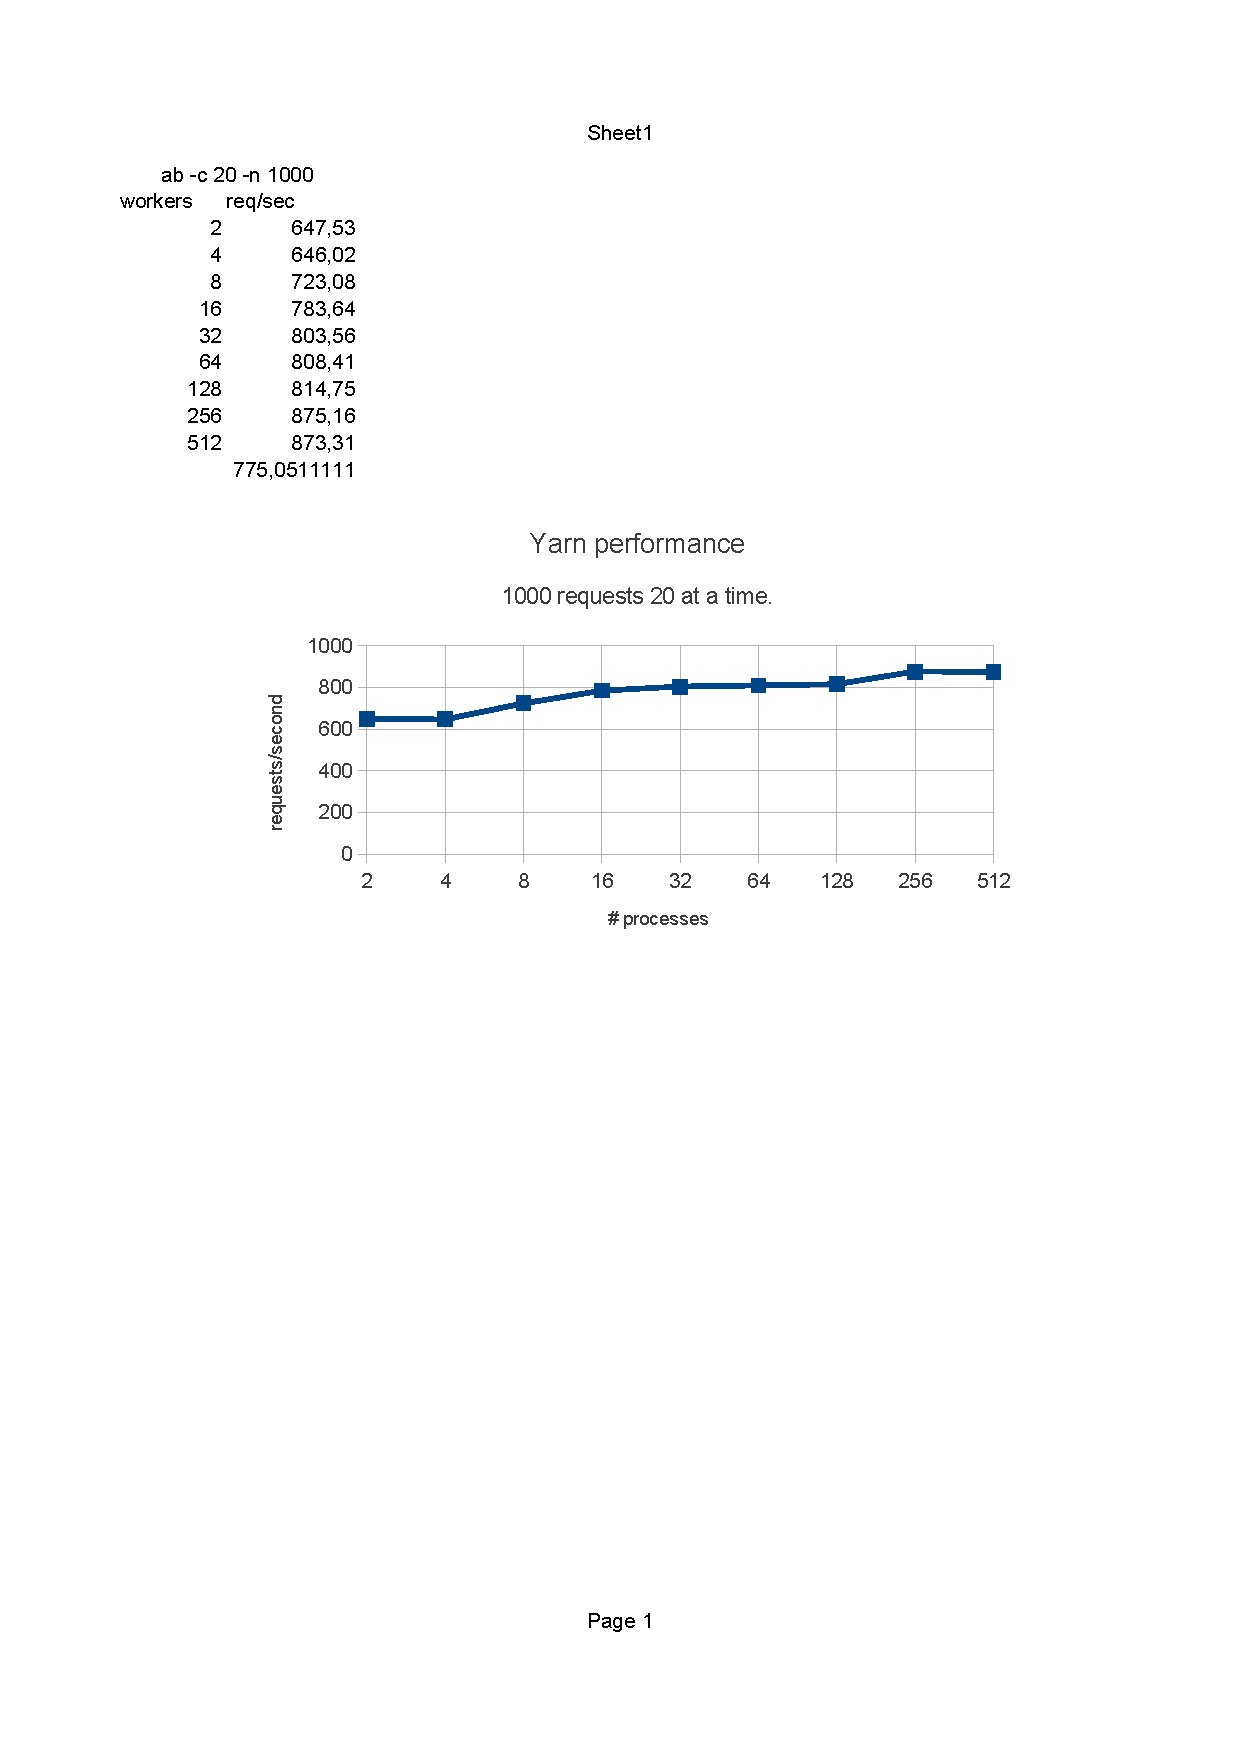
\includegraphics[width=1.0\textwidth]{results/optimal_workers.pdf}
  \caption{Yarn performance}
  \label{optwork}
\end{figure}

Test runs above 256 processes bogged the computer down and were not included.
The result of this was, context-switching and memory usage exceeded the
capabilities of the system. The best result was achieved with 32 worker
processes which maxed at 808 req/sec, and on average Yarn performed 706 req/sec. The
test consisted of making 2000 requests, 200 at a time, to Yarn serving a
simple Rack application (test\_objects/config.ru).

\subsection{Yarn Vs. Other Ruby Webservers}

\begin{figure}[htb]
  \centering
  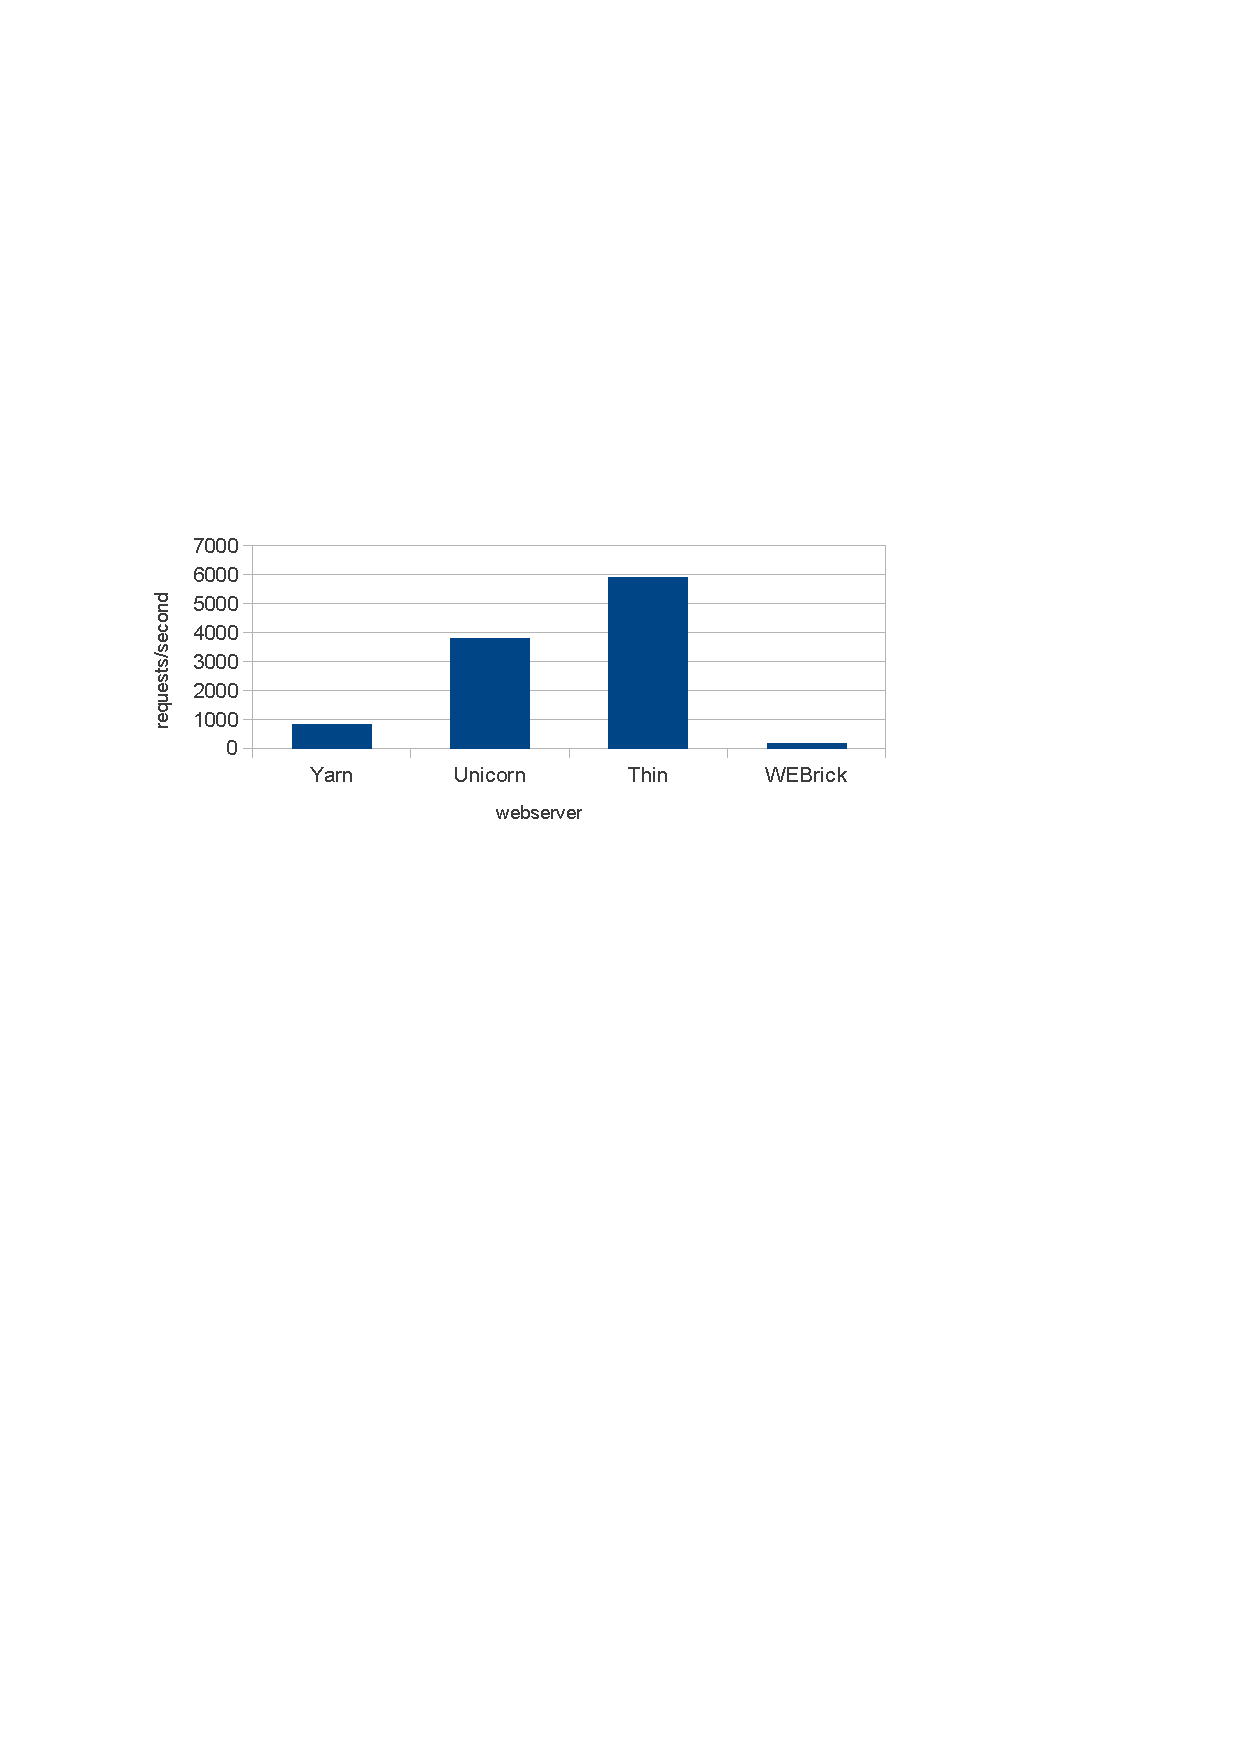
\includegraphics[width=1.0\textwidth]{benchmark/static.pdf}
  \caption{Yarn performance}
  \label{optwork}
\end{figure}

\begin{figure}[htb]
  \centering
  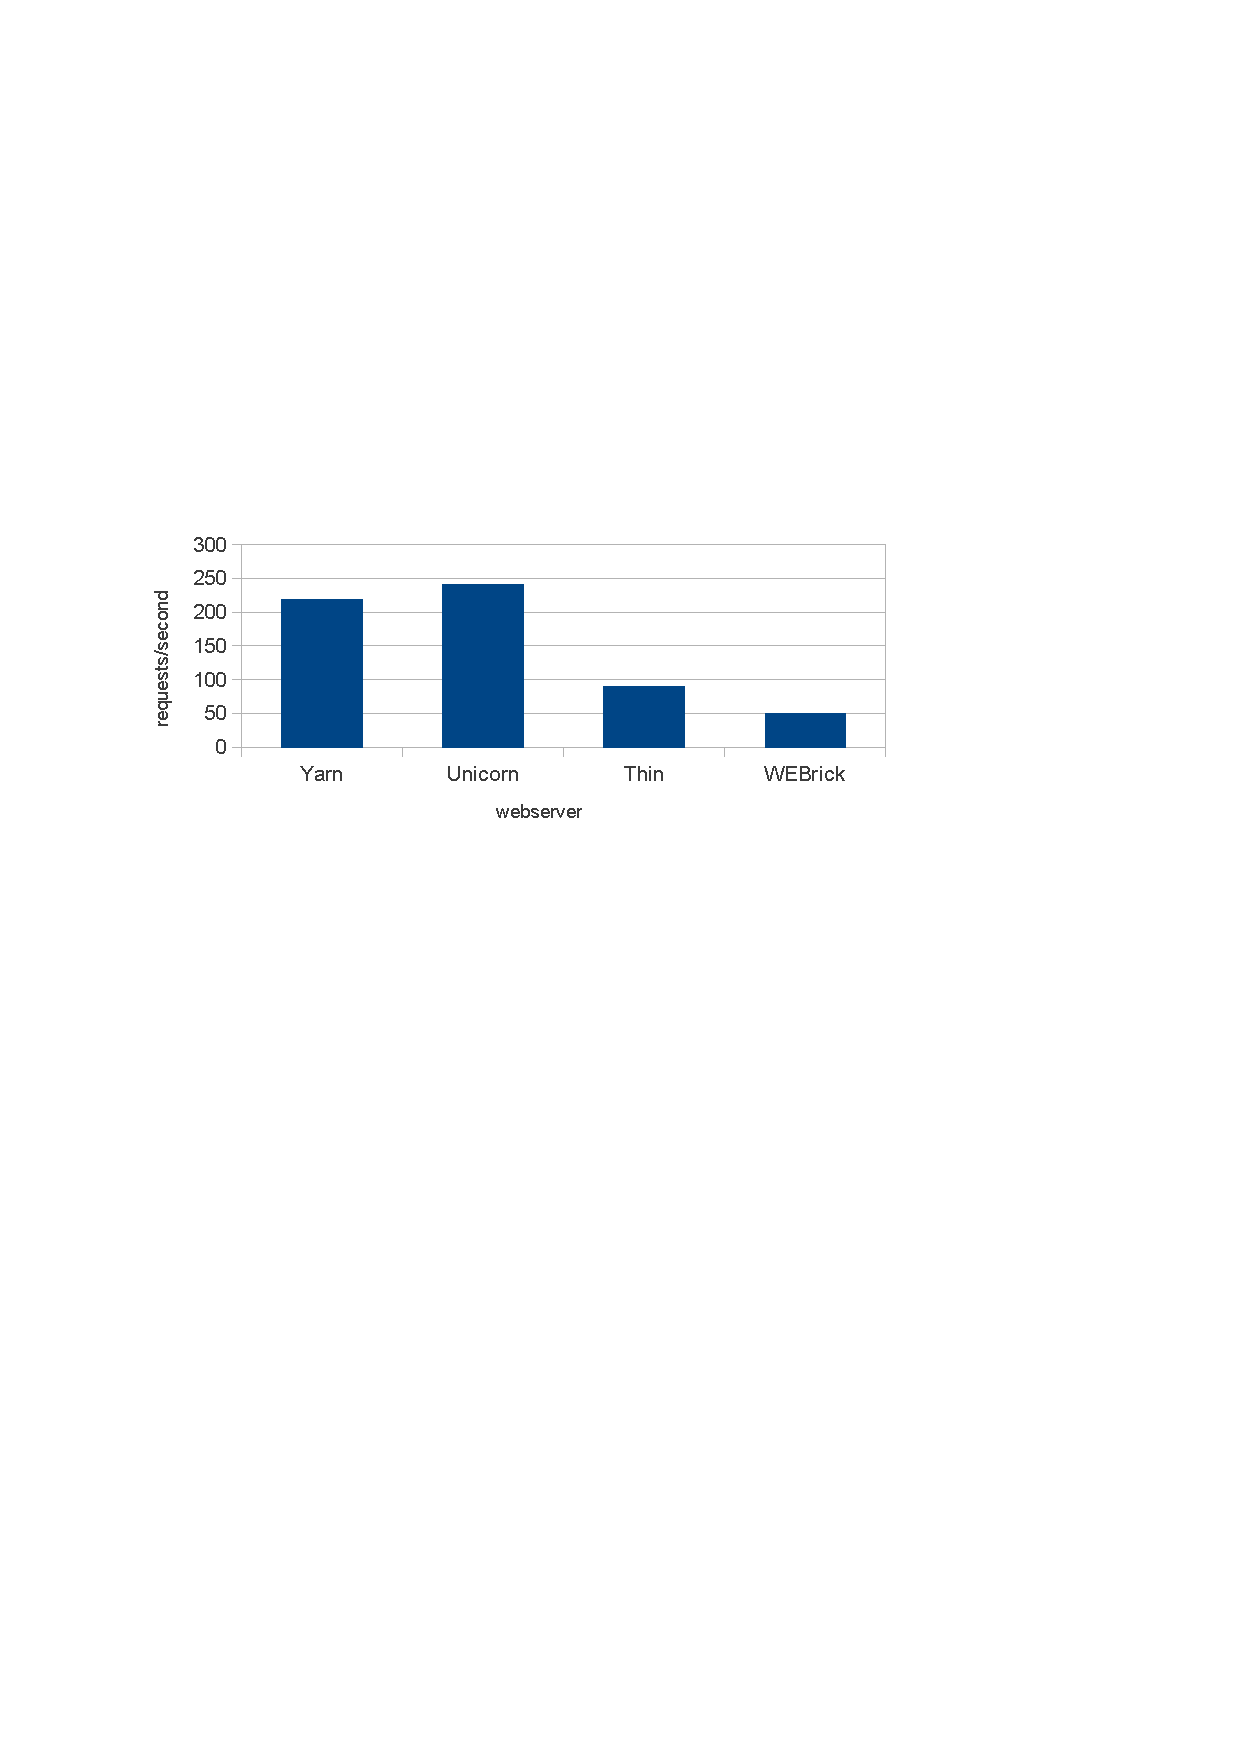
\includegraphics[width=1.0\textwidth]{benchmark/cpu.pdf}
  \caption{Yarn performance}
  \label{optwork}
\end{figure}
